\chapter{Progettazione}
\label{ch:progettazione}

Il seguente lavoro di tesi riguarda l'impiego di tecniche innovative nel campo dell'IoT, nello specifico, la progettazione e la valutazione di reti di monitoraggio mesh indoor basate sul nuovo standard fornito da Bluetooth SIG, la tecnologia \textit{\texttt{Bluetooth Mesh}}.
A tale standard è stato accostato come tecnologia di supporto uno standard ampiamente diffuso, ovvero lo standard \textit{\texttt{IEEE 802.11}}. L'impiego sul medesimo nodo di entrambe le tecnologie garantisce sia la comunicazione con i nodi in grado di supportare solo uno dei due standard sia la possibilità di scegliere il canale da utilizzare in base alle situazioni dell'ambiente circostante.\\

\noindent Il seguente progetto di tesi ha come obiettivo quello di garantire la comunicazione tra dispositivi IoT in un ambiente indoor (in qualsiasi situazione) e allo stesso tempo cercando di minimizzare i consumi energetici. La scelta è ricaduta sulle due tecnologie preannunciate poiché al giorno d'oggi esse risultano presenti in qualsiasi tipologia di apparato d'uso quotidiano. \\
Al fine di salvaguardare i consumi energetici la tecnologia prevalentemente utilizzata come mezzo di comunicazione riguarda Bluetooth Mesh, mentre si ricorre alla tecnologia di supporto solo nel caso in cui una comunicazione non andasse a buon fine attraverso la tecnologia prediletta.\\
Una volta implementato il codice che consentisse di operare come preannunciato si è passati alla fase di valutazione del modello realizzato. La valutazione in merito al comportamento della rete ha riguardato sia il variare della distanza tra mittente e destinatario sia il variare del carico di lavoro. Con carico di lavoro si intende la frequenza con cui vengono immessi i messaggi nella rete e ai fini di tale valutazione è molto importante il metodo di comunicazione request-response. Utilizzando tale modello, un messaggio viene definito perso nel momento in cui non sopraggiunge al Client la risposta da parte del Server.\\

\begin{figure}[!ht]
    \centering
    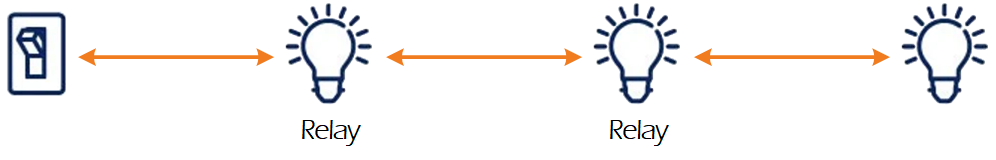
\includegraphics[width = \textwidth]{images/Mesh_network.png}
    \caption{rete Bluetooth Mesh}
    \label{fig:mesh_network}
\end{figure}

\noindent La comunicazione tra i nodi della rete può avvenire tramite diverse tipologie di messaggi (\ref{subsub:messaggi}). Tra le tipologie supportate si è ricorso all'impiego di messaggi di tipo \texttt{SET}, poiché oltre a modificare lo stato del nodo, sono in grado di supportare il meccanismo di acknowledgment. Vale a dire che alla ricezione di un tale messaggio, il nodo dopo aver attuato il cambio di stato comunicato provvede ad inviare al mittente una conferma di ricezione dell'operazione da svolgere, avvalendosi del messaggio di tipo \texttt{STATUS}.\\

\noindent Con l'impiego di questa modalità di comunicazione, garantita direttamente dallo standard Bluetooth Mesh, si riesce a soddisfare il criterio di comunicazione bidirezionale, ma con l'aumentare del carico di lavoro all'interno della rete e con la latenza in continua ascesa sono venute fuori alcune problematiche legate proprio alla tipologia di messaggio utilizzato. \\ % Invio di un mex alla stessa destinazione solo dopo aver atteso la scadenza del timer o la ricezione del ack 
Tale tipologia di messaggi (con acknowledgment), prevede la configurazione di un parametro ``timeout'' al fine di determinare l'evento di perdita e procedere con una nuova trasmissione. Tale implementazione prevede che finché non viene innescato tale evento o non viene ricevuta la conferma di ricezione, il sistema impedisce l'invio di ulteriori messaggi alla medesima destinazione. Solo al verificarsi di una delle due situazioni è possibile inviare un nuovo messaggio a tale indirizzo. \\
Ai fini di questo lavoro tale situazione risulta essere troppo stringente, allora si è provveduto ad implementare un meccanismo specifico evitando di utilizzare il meccanismo di acknowledgment fornito dallo standard.\\ 
Il meccanismo proposto prevede lato mittente l'utilizzo di semplici messaggi di tipo \texttt{SET} (senza acknowledgment), per innescare un cambiamento di stato nel dispositivo destinatario, e un meccanismo di risposta personalizzato lato destinatario. Il destinatario, alla ricezione di un determinato messaggio, dovrà elaborarlo e individuare il valore relativo allo stato da attuare, dopodiché procedere con la creazione di un messaggio di risposta (di tipo \texttt{STATUS}) contenente tale valore da rispedire al mittente. Una volta inviata la risposta, procedere con l'attuazione del cambiamento di stato comunicato.\\ % Failed to send Generic Set message --- Busy sending message to DST

\noindent La predetta configurazione (con l'impiego della sola tecnologia BLE Mesh) è stata utilizzata nella prima fase di test. Analizzando i risultati ottenuti è stata individuata un'elevata perdita di pacchetti per via delle interferenze, della congestione dovuta al carico di lavoro elevato e per via delle specifiche imposte da tale standard. Il fattore perdite è stato fondamentale per confermare l'introduzione di una tecnologia di supporto (la tecnologia 802.11) al fine di garantire la comunicazione tra i nodi della rete in qualsiasi circostanza.\\
Inizialmente, si è pensato di adottare l'approccio Wi-Fi Mesh, il modo da avere il medesimo modello di funzionamento per entrambe le tecnologie. Però, dopo opportune osservazioni è venuto fuori che adoperare sul medesimo ruolo sia la tecnologia BLE Mesh sia la tecnologia Wi-Fi Mesh risultava infattibile in termini di memoria. Il modus operandi legato a tali tecniche prevede una quantità di memoria nettamente maggiore di quella di cui risultano dotati dei semplici dispositivi a nostra disposizione (\texttt{ESP32}). \\
Poiché tali dispositivi non supportano neppure la modalità di rete hoc, si è ricorso all'utilizzo del tradizionale Wi-Fi e quindi con l'introduzione di un'entità esterna avente la funzione di router. Poiché il raggio di copertura garantito dalla tecnologie Wi-Fi risulta essere maggiore rispetto a quello del Bluetooth, è stato possibile utilizzare un solo dispositivo router per garantire la comunicazione, con tale tecnologia, tra tutti i appartenenti alla rete.\\

\begin{figure}[!ht]
    \centering
    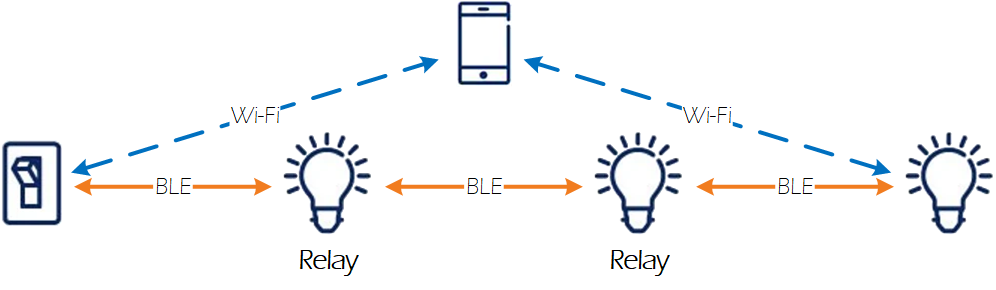
\includegraphics[width = \textwidth]{images/BLE_WiFi.png}
    \caption{rete Bluetooth mesh - WiFi}
    \label{fig:mesh_network_wifi}
\end{figure}

\noindent Determinate le tecnologie da impiegare nel seguente lavoro è stato necessario definire come farle interagire tra loro al fine di diminuire la perdita di pacchetti e allo stesso tempo di salvaguardare i consumi energetici.\\
Per fronteggiare tale situazione si è pensato di utilizzare come tecnologia preferita, lo standard Bluetooth Mesh e nel momento in cui si identifica la perdita di un pacchetto provvedere a ritrasmetterlo utilizzando la tecnologia di supporto (più dispendioso dal punto di vista energetico). In tal modo, con l'alternanza delle due tecnologie si allevia il carico di lavoro sulla tecnologia preferita garantendo sempre la comunicazione tra i nodi della rete.\\

\begin{figure}[!ht]
    \centering
    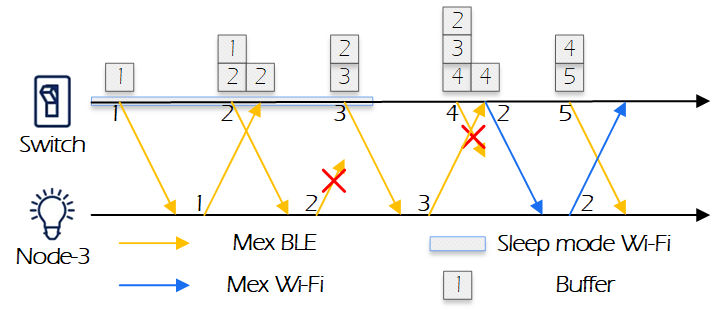
\includegraphics[width = \textwidth]{images/Algoritmo_dinamico.png}
    \caption{Algoritmo dinamico per utilizzare la tecnologia BLE Mesh e Wi-Fi}
    \label{fig:algoritmo dinamico}
\end{figure}

\noindent Conclusa l'implementazione dei nodi in base alle specifiche descritte, ovvero con l'impiego del doppio stack protocollare (BLE + Bluetooth Mesh e WiFi), sono stati eseguiti dei test posizionando i nodi così come descritto dalla figura \ref{fig:rete_mesh}. In segutio tali test sono stati analizzati e confrontati con i risultati ottenuti utilizzando solo la tecnologia Bluetooth.\\

\noindent Come preannunciato, il test prevede l'analisi del carico di lavoro che la rete è in grado di supportare e per studiare tale comportamento al variare di determinati parametri, è stato necessario comunicare ai nodi delle configurazioni da rispettare durante tale simulazione. Le configurazioni consentono di variare la frequenza con cui immettere i messaggi nella rete e il nodo destinatario di tali messaggi. Per fare tutto ciò senza dover ogni volta modificare il codice e caricarlo sui singoli nodi, si è pensato di strutturate il funzionamento di un nodo affinché potesse essere in grado di ricevere tali configurazioni e comportarsi di conseguenza.\\
Il metodo definito per comunicare al nodo il comportamento da assumere è basato su una comunicazione seriale. Avvalendosi di tale comunicazione è possibile indicare, tramite una regola, le informazioni necessarie al fine di configurare il nodo, avviare la simulazione ed ottenere in output il log di tale test.\\
Il processo di configurazione riguarda solo un nodo all'interno della rete, identificato con il nome di client.\\
Per assicurarsi questa comunicazione e fare in modo di modificare il comportamento di un nodo in tempo reale, senza dover reinstallare il software e riavviare l'intero processo di configurazione della rete, si è pensato all'impiego di un dispositivo \texttt{UART}\footnote{\textit{Universal Asynchronous Receiver-Transmitter}, un dispositivo hardware utilizzato per far dialogare tramite porta seriale un dispositivo di input/output con il nodo client}.\\

\begin{figure}[!ht]
    \centering
    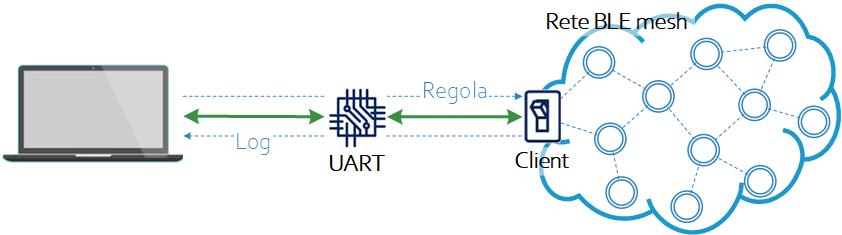
\includegraphics[width = \textwidth]{images/Uart.png}
    \caption{Architettura Rete BLE mesh - Test}
    \label{fig:mesh_network_uart}
\end{figure}

\noindent L'impiego di semplici dispositivi dotati di non molta memoria (tra l'altro sfruttata al massimo per eseguire i due stack protocollari) ha portato alla creazione del log non sul nodo ma su un dispositivo esterno. Anche in tale circostanza il \texttt{UART} è stato di fondamentale importanza. Tramite questa comunicazione è stato possibile comunicare il verificarsi di ogni singolo evento di nostro interesse.\\

\noindent La creazione della rete mesh avviene come indicato in precedenza, attraverso il processo di provisioning (sezione \ref{sec:provisioning}) e quindi prevede l'utilizzo di un provisioner. A tal proposito è stato adoperando uno smartphone con su installata un'apposita applicazione che consentisse la creazione, la configurazione e la gestione della rete mesh. Una volta creata la rete e configurati tutti i nodi è possibile procedere con l'esecuzione della di test relativa ai parametri comunicati.\\
Con l'impiego di entrambe le tecnologie, il dispositivo una volta entrato a far parte della rete mesh, non ha concluso la fase di configurazione ma procede con la sottoscrizione ad una determinata rete wifi, utilizzata solo per trasmettere i messaggi (denominati come `persi' con la tecnologia BLE mesh) tra i nodi della rete. \\
Solo dopo aver attivato entrambe le tecnologie, la fase di configurazione risulta essere terminata, ed è possibile procedere con la fase di test vera e propria.\\

